
\documentclass[aspectratio=169, handout]{beamer}

%\usepackage[table]{xcolor}
\mode<presentation> {
\setbeamercovered{transparent}
  \usetheme{Boadilla}

%  \usetheme{Pittsburgh}
%\usefonttheme[2]{sans}
\renewcommand{\familydefault}{cmss}
%\usepackage{lmodern}
%\usepackage[T1]{fontenc}
%\usepackage{palatino}
%\usepackage{cmbright}
\usepackage{bm}
\usepackage{listings}
\useinnertheme{rectangles}
}
\lstset{%
  language=R,
  basicstyle=\ttfamily\small,
  keywordstyle=\color{blue},
  commentstyle=\color{gray},
  stringstyle=\color{darkpurple},
  breaklines=true,
  numbers=left,
  numberstyle=\tiny,
  frame=single,
  framerule=0.5pt,
}
\usepackage{amsmath}
\setbeamercolor{normal text}{fg=black}
\setbeamercolor{structure}{fg= blue}
\definecolor{trial}{cmyk}{1,0,0, 0}
\definecolor{trial2}{cmyk}{0.00,0,1, 0}
\definecolor{darkgreen}{rgb}{0,.4, 0.1}
\definecolor{darkpurple}{rgb}{0.4, 0, 0.6}
\usepackage{array}
\beamertemplatesolidbackgroundcolor{white}  \setbeamercolor{alerted
text}{fg=darkpurple}
\usepackage{tcolorbox}
\setbeamertemplate{caption}[numbered]\newcounter{mylastframe}

\font\domino=domino
\def\die#1{{\domino#1}}
\usepackage{tikz}
\usetikzlibrary{arrows,positioning}
\usepackage{colortbl}

\usepackage{lipsum}

 \newenvironment{changemargin}[3]{%
 \begin{list}{}{%
 \setlength{\topsep}{0pt}%
 \setlength{\leftmargin}{#1}%
 \setlength{\rightmargin}{#2}%
 \setlength{\topmargin}{#3}%
 \setlength{\listparindent}{\parindent}%
 \setlength{\itemindent}{\parindent}%
 \setlength{\parsep}{\parskip}%
 }%
\item[]}{\end{list}}

\usecolortheme{lily}

\newtheorem{com}{Comment}
\newtheorem{lem} {Lemma}
\newtheorem{prop}{Proposition}
\newtheorem{condition}{Condition}
\newtheorem{thm}{Theorem}
\newtheorem{defn}{Definition}
\newtheorem{cor}{Corollary}
\newtheorem{obs}{Observation}
 \numberwithin{equation}{section}
 
\makeatletter
\def\beamerorig@set@color{%
  \pdfliteral{\current@color}%
  \aftergroup\reset@color
}
\def\beamerorig@reset@color{\pdfliteral{\current@color}}
\makeatother
\setbeamertemplate{navigation symbols}{}

\useoutertheme{miniframes}
\title[PLSC 30700]{Linear Models Lecture 3: Estimation of the Linear Projection Model}

\author{Robert Gulotty}
\institute[Chicago]{University of Chicago}


\begin{document}

\begin{frame}
\maketitle
\end{frame}





\section{Derivation of OLS}

\begin{frame}{Deriving the OLS estimator}
\begin{itemize}
\item Recall, geometry can work in populations or samples.
\item In the following slides we will derive 
\begin{itemize} 
\item the OLS slope estimator $\bm{\hat{\beta}}$,
\item the OLS estimator for error variance,
\item Decomposition of OLS (Analysis of Variance), with $R^2$
\end{itemize}
\item Next time, the FWL Theorem.
\end{itemize}
\end{frame}

\begin{frame}{Review: From Population to Inference}
\begin{itemize}
\item The CEF and linear projection are facts about \textbf{populations}---we derived $\beta=[\mathbb{E}[XX']]^{-1}\mathbb{E}[XY]$ last time.\pause
\item But we don't observe populations. We observe \textbf{samples}.\pause
\end{itemize}
\vspace{0.5em}
\begin{center}
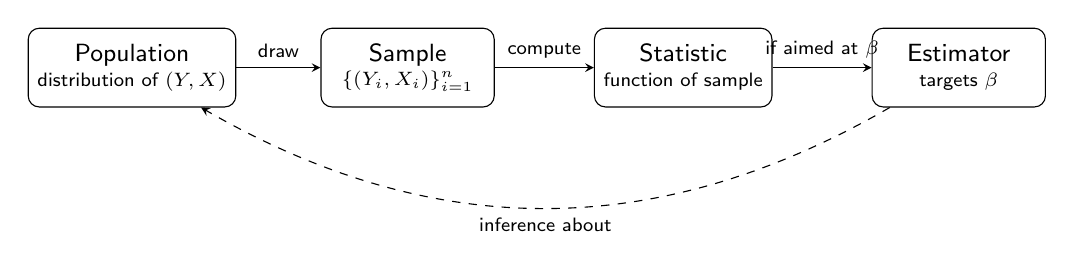
\begin{tikzpicture}[>=stealth, node distance=2.2cm,
  box/.style={draw, rounded corners, minimum height=1cm, minimum width=2.2cm, align=center, font=\small}]
\node[box] (pop) {Population\\[-2pt]{\scriptsize distribution of $(Y,X)$}};
\node[box, right of=pop, node distance=3.5cm] (sample) {Sample\\[-2pt]{\scriptsize $\{(Y_i,X_i)\}_{i=1}^n$}};
\node[box, right of=sample, node distance=3.5cm] (stat) {Statistic\\[-2pt]{\scriptsize function of sample}};
\node[box, right of=stat, node distance=3.5cm] (est) {Estimator\\[-2pt]{\scriptsize targets $\beta$}};
\draw[->] (pop) -- node[above, font=\scriptsize] {draw} (sample);
\draw[->] (sample) -- node[above, font=\scriptsize] {compute} (stat);
\draw[->] (stat) -- node[above, font=\scriptsize] {if aimed at $\beta$} (est);
\draw[->, dashed] (est) to[bend left=30] node[below, font=\scriptsize] {inference about} (pop);
\end{tikzpicture}
\end{center}
\vspace{0.3em}
\begin{itemize}
\item A \alert{statistic} is any function of the sample (e.g.\ $\bar{Y}$, $s^2$, a histogram).
\item An \alert{estimator} is a statistic designed to estimate a population parameter.
\end{itemize}
\end{frame}

\begin{frame}{Samples}
\begin{itemize}
\item We estimate the projection coefficient $\beta$ with measurements of $(Y,X)$, a \emph{sample}.\pause
\item $\{(Y_i, X_i):\ i\in1,\ldots,\ n\}$, is the sample, governed by the distribution of $(Y,X)$.\pause
\item From the next slide forward, $\bm{X}$ is going to be a matrix, and we will use lower case for vectors e.g. $\bm{e}$.
\end{itemize}
\end{frame}

\begin{frame}{Identically Distributed.}
\begin{itemize}
\item Main approach is to assume homogeneity: $\{(Y_i, \bm{x}_i):\ i\in1,\ldots,\ n\}$ are identically distributed.
\begin{align*}
\begin{bmatrix}Y_1\\ \vdots \\Y_n\end{bmatrix}&=\beta_1\begin{bmatrix}1 \\\vdots\\1\end{bmatrix}+\beta_2 \begin{bmatrix}X_{21} \\ \vdots \\ X_{2n}\end{bmatrix}+\beta_3 \begin{bmatrix}X_{31} \\\vdots\\ X_{3n} \end{bmatrix}+\begin{bmatrix}e_1 \\ \vdots \\ e_n\end{bmatrix}
\\
&=\begin{bmatrix}1 &X_{21}& X_{31} \\\vdots &\vdots& \vdots  \\1  &X_{2n}& X_{3n} \end{bmatrix} \begin{bmatrix} \beta_1\\ \beta_2 \\ \beta_3 \end{bmatrix}+\begin{bmatrix}e_1 \\ \vdots \\ e_n\end{bmatrix}\\
\bm{y}&=\bm{X}\bm{\beta}+\bm{e}
\end{align*}
\item Note, $\mathbb{E}[Y_1|\bm{x}_1]\neq \mathbb{E}[Y_2|\bm{x}_2]$ in general (different covariates imply different conditional means).
\end{itemize}
\end{frame}


\begin{frame}{Least Squares Estimator}
\begin{itemize}
\item The linear projection coefficient $\beta$ is the minimizer of the expected squared error 
$$S(\beta)=\mathbb{E}[(Y-\bm{x}'\beta)^2]$$
\item The \emph{moment estimator} of $S(\beta)$ is the sample average:
$$\hat{S}(\beta)=\frac{1}{n}\sum_{i=1}^{n}(Y_i-\bm{x}_i'\beta)^2$$
\item $\sum_{i=1}^{n}(Y_i-\bm{x}_i'\beta)^2$ is called SSE($\beta$), the \textbf{sum of squared errors}.
\item The estimator $\hat{\beta}$ is the minimizer of $\hat{S}(\beta)$, as well as the minimizer of the SSE.
\item $\hat{\beta}$ is called the least squares estimator, sometimes written $\hat{\beta}_n$.
\end{itemize}
\end{frame}



\begin{frame}{The Plan}
\begin{itemize}
\item We have a population quantity $\beta$ and a sample objective $\hat{S}(\beta)$. Now we need to:
\begin{enumerate}
\item \textbf{Find} $\hat{\beta}$: minimize SSE using matrix calculus.\pause
\item \textbf{Understand} $\hat{\beta}$ geometrically: projection matrices $\bm{P}$ and $\bm{M}$.\pause
\item \textbf{Quantify uncertainty}: estimate $\sigma^2$ from residuals, then get standard errors for $\hat{\beta}$.
\end{enumerate}\pause
\item Note, residuals $\neq$ disturbances.  The former is estimated.
\end{itemize}
\end{frame}

\begin{frame}{Finite Sample Assumptions of OLS estimator}
\begin{itemize}
\item Assumption 1: The random variables $\{(Y_1,\ \bm{x}_1),\ (Y_2,\ \bm{x}_2), \ldots, (Y_n,\ \bm{x}_n)\}$ are independent and identically distributed.
\item Assumption 2: $Y=\bm{x}'\bm{\beta}+e$, where $\mathbb{E}(e|\bm{x})=0$.
\item Assumption 3: $\mathbb{E}(\bm{x}\bm{x}')>0$ (with probability 1).
\item Assumption 4*: $\mathbb{E}[e^2|\bm{x}]=\sigma^2(\bm{x})=\sigma^2$. 
\end{itemize}
\end{frame}


\begin{frame}{Derivation of Least Squares Estimator}
\begin{itemize}
\item The functional form of the least squares estimator can be derived via multivariate calculus.
\item We look for a minimum of SSE($\beta$).
\item Take first derivatives to calculate first-order conditions and locate the critical values.
\item Then we check we have the global minimum, by using the fact that positive definite matrices represent convex functions.
\end{itemize}
\end{frame}


\begin{frame}{Calculus Derivation of Least Squares Estimator}
\begin{align*}
SSE(\beta)&=(\bm{y}-\bm{X\beta})'(\bm{y}-\bm{X\beta}) \tag{Definition of $\bm{e}$}\\
&=(\bm{y}'-\bm{\beta'X'})(\bm{y}-\bm{X\beta}) \tag{Transpose rules}\\
&=\bm{y}'\bm{y}-\bm{\beta'X'y}-\bm{y}'\bm{X\beta}+\bm{\beta'X'X\beta}  \tag{Distributive property}\\
\min_{\bm{\beta}} SSE(\beta)&=\min_{\bm{\beta}}\ \underbrace{\bm{y}'\bm{y}}_{\text{constant}}\,-\,\underbrace{2\bm{y}'\bm{X\beta}}_{\text{linear in }\bm{\beta}}\,+\,\underbrace{\bm{\beta'X'X\beta}}_{\text{quadratic form}}
\end{align*}
\end{frame}

\begin{frame}{Calculus Derivation of Least Squares Estimator}
\begin{align*}
\frac{\partial\bm{y}'\bm{y}-\bm{\beta'X'y}-\bm{y}'\bm{X\beta}+\bm{\beta'X'X\beta}}{\partial\bm{\beta}}&=\bm{0}-\bm{X'y}-\bm{X'y}+(\bm{X'X+X'X})\bm{\hat{\beta}}\\
&=-2\bm{X}'\bm{y}+2\bm{X}'\bm{X}\bm{\hat{\beta}} \tag{Symmetric}\\
-2\bm{X}'\bm{y}+2\bm{X}'\bm{X}\bm{\hat{\beta}}&=\bm{0} \tag{find critical point}\\
\bm{X}'\bm{X}\bm{\hat{\beta}}&=\bm{X}'\bm{y}. \tag{normal equations}\\
\bm{\hat{\beta}}&=(\bm{X}'\bm{X})^{-1}\bm{X}'\bm{y} \tag{If $\bm{X}'\bm{X}$ can be inverted (A3).}
\end{align*}
\end{frame}

\begin{frame}{Second order condition}
Take second derivative, and check that it is positive
\begin{align*}
\frac{\partial -2\bm{X}'\bm{y}+2\bm{X}'\bm{X}\bm{\hat{\beta}}}{\partial \bm{\hat{\beta}'}}&=2(\bm{X}'\bm{X})'
\end{align*}
Which is positive so long as $\bm{X}'\bm{X}$ is positive definite (Assumption A3).\\
$\bm{\hat{\beta}}$ minimizes the sum of squared errors, assuming $\bm{X}$ is of full rank.
\end{frame}

\begin{frame}[fragile]{OLS in R: The Formula in Action}
\begin{lstlisting}
library(carData)
X <- cbind(1, Prestige$education, Prestige$income)
y <- Prestige$prestige

# The matrix formula from the slides:
solve(t(X) %*% X) %*% t(X) %*% y

# What lm() computes:
coef(lm(prestige ~ education + income, data=Prestige))
\end{lstlisting}
\vspace{1ex}
The two are identical: \texttt{lm()} implements $\hat{\beta}=(\bm{X'X})^{-1}\bm{X'y}$.
\end{frame}

\begin{frame}{Projection Matrix}
\begin{itemize}
\item There is a geometric interpretation for the minimization problem that uses the idea of ``projection''.
\item The following matrix is called a ``projection matrix'':
$$\bm{P}=\bm{X}(\bm{X}'\bm{X})^{-1}\bm{X}'$$
\item Intuition: $\bm{P}$ takes any vector in $\mathbb{R}^n$ and drops it onto the column space of $\bm{X}$---the closest point that can be written as $\bm{X}b$ for some $b$.\pause
\item The key payoff: $\bm{P}\bm{y}=\bm{X}\bm{\hat{\beta}}=\bm{\hat{y}}$. This is why $\bm{P}$ is also called the ``hat matrix''---it puts the hat on $\bm{y}$.
\end{itemize}
\end{frame}

\begin{frame}{Properties of the Projection Matrix}
\begin{itemize}
\item $\bm{P}$ leaves anything already in the column space alone:\pause
\begin{itemize}
\item $\bm{P}\bm{X}=\bm{X}(\bm{X}'\bm{X})^{-1}\bm{X}'\bm{X}=\bm{X}$
\item If $\bm{X}=[\bm{X}_1\ \bm{X}_2]$, then $\bm{P}\bm{X}_1=\bm{X}_1$.
\end{itemize}\pause
\item $\bm{P}$ is \textbf{symmetric}: $\bm{P}=\bm{P}'$.\pause
\item $\bm{P}$ is \textbf{idempotent}: $\bm{P}\bm{P}=\bm{P}$.
\pause
\item These two properties (symmetric + idempotent) will do a lot of work for us in the rest of the course.
\end{itemize}
\end{frame}





\begin{frame}{Projection onto column of 1}
\begin{itemize}
\item If $\bm{X}=\bm{1}$, then
$\bm{P}_1=\bm{1}(\bm{1}'\bm{1})^{-1}\bm{1}'=\frac{1}{n}\bm{1}\bm{1}'$
\item So if we project $\bm{y}$ onto $\bm{P}_1$, we get a vector repeating the sample mean:
\begin{align*}
\bm{P}_1\bm{y}&=\frac{1}{n}\bm{1}\bm{1}'\bm{y}=\bm{1}\cdot\frac{1}{n}\sum_{i=1}^nY_i=\bm{1}\bar{Y}
\end{align*}
\item \textbf{Takeaway:} The simplest regression (intercept only) projects $\bm{y}$ onto the sample mean. Every additional regressor refines this projection.
\item The annihilator $\bm{M}_1\bm{y}=\bm{y}-\bm{1}\bar{Y}$ \emph{demeans} $\bm{y}$---it removes the part explained by the intercept.
\end{itemize}
\end{frame}

\begin{frame}{Orthogonal Projection}
\begin{itemize}
\item The following matrix is called an "orthogonal projection matrix", or the Annihilator Matrix.
\begin{align*}
\bm{M}&=\bm{I}_n-\bm{P}\\
&=\bm{I}_n-\bm{X}(\bm{X}'\bm{X})^{-1}\bm{X}'
\end{align*}
\item $\bm{M}$ and $\bm{X}$ are orthogonal:
\begin{align*}
\bm{MX}&=(\bm{I}_n-\bm{P})\bm{X}\\
&=\bm{X}-\bm{P}\bm{X}\\
&=\bm{X}-\bm{X}\\
&=0
\end{align*}
\item We can define the residuals from projecting onto a column of 1s: $\bm{M}_1\bm{y}=\bm{y}-\bm{1}\bar{Y}$, this demeans $\bm{y}$.

\end{itemize}
\end{frame}

\begin{frame}{Relationship between residuals and disturbances}

\begin{align*}
\bm{\hat{e}}&=\bm{y}-\bm{\hat{y}}\\
&=\bm{y}-\bm{X\hat{\beta}}\\
&=\bm{y}-\bm{Py}\\
&=\bm{My}\\
&=\bm{M}(\bm{X\beta}+\bm{e})\\
&=\bm{M}\bm{X\beta}+\bm{M}\bm{e}\\
&=\bm{M}\bm{e}
\end{align*}

\end{frame}

\begin{frame}[fragile]{Projection and Residuals in R}
\begin{lstlisting}
mod <- lm(prestige ~ education + income, data=Prestige)
X <- cbind(1, Prestige$education, Prestige$income)
P <- X %*% solve(t(X) %*% X) %*% t(X)
M <- diag(nrow(X)) - P

# P*y = fitted values
all.equal(as.vector(P %*% y), fitted(mod))  # TRUE

# M*y = residuals
all.equal(as.vector(M %*% y), resid(mod))   # TRUE
\end{lstlisting}
\vspace{1ex}
$\bm{P}$ and $\bm{M}$ are used by R to compute \texttt{fitted()} and \texttt{resid()}.
\end{frame}

\section{Estimation of \texorpdfstring{$\sigma^2$}{the error variance}}

\begin{frame}{Where We Stand}
\begin{itemize}
\item We have $\hat{\beta}=(\bm{X'X})^{-1}\bm{X'y}$ and the geometry behind it ($\bm{P}$, $\bm{M}$).\pause
\item But how precise is $\hat{\beta}$? To answer that, we need $\text{Var}(\hat{\beta}|\bm{X})=\sigma^2(\bm{X'X})^{-1}$.\pause
\item Problem: $\sigma^2$ is \emph{unknown}---it's a population quantity, just like $\beta$.\pause
\item So we need a second estimator, $s^2_e$, built from the residuals. This is step 3.
\end{itemize}
\end{frame}

\begin{frame}{Why Does Projection Help?}
\begin{itemize}
\item We want to estimate the systematic part $\bm{X\beta}$. Two candidates:
\begin{enumerate}
\item Use $\bm{y}$ itself (just report the raw data).
\item Use $\bm{Py}=\bm{\hat{y}}$ (the projection onto the column space of $\bm{X}$).
\end{enumerate}\pause
\item Compare their variances as estimators of $\bm{X\beta}$:
\begin{align*}
\text{Var}(\bm{y}|\bm{X})&=\sigma^2\bm{I}\\
\text{Var}(\bm{Py}|\bm{X})&=\sigma^2\bm{P}
\end{align*}\pause
\item The difference is $\sigma^2(\bm{I}-\bm{P})=\sigma^2\bm{M}$, which is positive semi-definite.
\item So $\text{Var}(\bm{y})\geq \text{Var}(\bm{Py})$: projection \emph{removes noise} without distorting the signal, because $\bm{PX\beta}=\bm{X\beta}$.
\end{itemize}
\end{frame}


\begin{frame}{Variance of the regression errors}
\begin{itemize}
\item We want to measure the precision of our regression estimates.
\item The error (or disturbance) of an observation is the deviation of a value from its theoretical mean, cannot be observed.
\item The coefficients inherit that uncertainty from the theoretical model.
\item Our estimates have additional uncertainty, related to the fact we only have a sample.
\item Residuals are the difference between observations and estimates, can be observed.
\end{itemize}
\end{frame}


\begin{frame}{The Bane of Statistics: We Never See the Errors}
\begin{center}
\begin{tabular}{l@{\hskip 2em}l@{\hskip 2em}l}
& \textbf{Disturbance $e_i$} & \textbf{Residual $\hat{e}_i$}\\
\hline
Definition & $Y_i - \bm{x}_i'\beta$ & $Y_i - \bm{x}_i'\hat{\beta}$\\[4pt]
Depends on & population $\beta$ & estimated $\hat{\beta}$\\[4pt]
Observable? & \alert{No} & Yes\\[4pt]
Distribution & $E[e_i|\bm{X}]=0$,\ $\text{Var}(e_i)=\sigma^2$ & $\hat{e}_i = \bm{M}_i\bm{e}$ (a linear combo of \emph{all} $e_j$'s)\\
\end{tabular}
\end{center}
\vspace{0.5em}
\begin{itemize}
\item We showed that $\bm{\hat{e}}=\bm{Me}$: each residual is a \emph{filtered} version of the true disturbances, not a direct copy.\pause
\item This means MSE (computed on residuals) $\neq$ true error variance. We will need a degrees-of-freedom correction ($n-k$) to fix this.
\end{itemize}
\end{frame}



\begin{frame}{Estimating the Disturbance Variance: First Attempt}
\small
\begin{itemize}
\item Terminology note: \emph{disturbance}, \emph{error}, and \emph{noise} all refer to $e_i = Y_i - \bm{x}_i'\beta$. We use them interchangeably; the key point is that $e_i$ is \textbf{unobservable}.\pause
\item Natural idea: plug the residuals $\hat{e}_i$ into the sample variance formula:
$$\hat{\sigma}^2=n^{-1}\bm{\hat{e}'\hat{e}}=n^{-1}(\bm{My})'(\bm{My})=n^{-1}\bm{y'My}=n^{-1}\bm{e'Me}$$
where the last step uses $\bm{M}=\bm{M'M}$ and $\bm{MX}=0$.\pause
\item But $\bm{\hat{e}'\hat{e}} \leq \bm{e'e}$, so residuals underestimate the true sum of squared errors:
\begin{align*}
n^{-1}\bm{e'e}-n^{-1}\bm{e'Me}=n^{-1}\bm{e'Pe}\geq 0
\end{align*}
because $\bm{P}$ is positive semi-definite.
\item Projection ``absorbs'' some of the disturbance into fitted values, so residuals understate the true noise.
\end{itemize}
\end{frame}


\begin{frame}{The Degrees-of-Freedom Correction}
\small
\begin{itemize}
\item Fix: divide by $n-k$ instead of $n$. Define $s^2_e=\bm{\hat{e}}'\bm{\hat{e}}/(n-k)$.
\item Proof that $s^2_e$ is unbiased for $\sigma^2$:
\begin{align*}
\bm{\hat{e}}'\bm{\hat{e}}&=\bm{e'M'Me}=\bm{e'Me} \tag{$\bm{M}$ symmetric, idempotent}\\
E[\bm{\hat{e}}'\bm{\hat{e}}|\bm{X}]&=E[\bm{e'Me}|\bm{X}]\\
&=E[\text{tr}(\bm{e'Me})|\bm{X}] \tag{scalar $=$ its own trace}\\
&=E[\text{tr}(\bm{Mee'})|\bm{X}] \tag{tr($\bm{ABC}$)=tr($\bm{CAB)}$}\\
&=\text{tr}(\bm{M}\, E[\bm{ee'}|\bm{X}]) \tag{$\bm{M}$ fixed given $\bm{X}$}\\
&=\text{tr}(\bm{M}\sigma^2\bm{I})=\sigma^2\text{tr}(\bm{M})=\sigma^2 (n-k) \tag{A4, tr($\bm{M}$)=$n-k$}
\end{align*}
\end{itemize}
\end{frame}



\begin{frame}{Standard Deviation vs.\ Standard Error}
\begin{center}
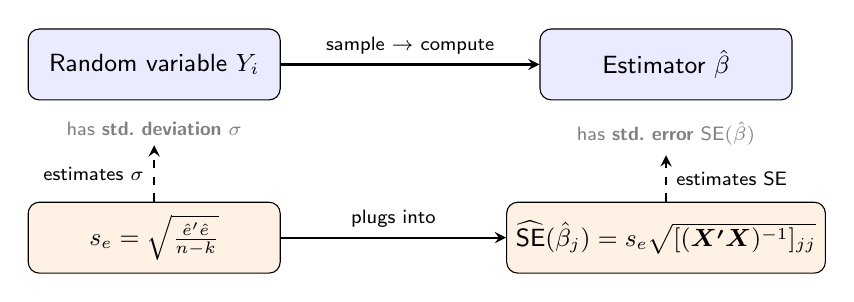
\begin{tikzpicture}[>=stealth,
  lvl/.style={draw, rounded corners, minimum width=3.2cm, minimum height=0.9cm, align=center, font=\small},
  arr/.style={->, thick}]
% Left column: the random variable level
\node[lvl, fill=blue!8] (rv) at (0,0) {Random variable $Y_i$};
\node[below=0.15cm of rv, font=\scriptsize, text=gray] (rvsd) {has \textbf{std.\ deviation} $\sigma$};

% Middle column: the estimator level
\node[lvl, fill=blue!8] (est) at (6.5,0) {Estimator $\hat{\beta}$};
\node[below=0.15cm of est, font=\scriptsize, text=gray] (estse) {has \textbf{std.\ error} $\text{SE}(\hat{\beta})$};

% Arrows
\draw[arr] (rv) -- node[above, font=\scriptsize] {sample $\to$ compute} (est);

% Lower row: what we estimate each with
\node[lvl, fill=orange!10] (shat) at (0,-2.2) {$s_e = \sqrt{\frac{\hat{e}'\hat{e}}{n-k}}$};
\node[lvl, fill=orange!10] (sehat) at (6.5,-2.2) {$\widehat{\text{SE}}(\hat{\beta}_j)=s_e\sqrt{[(\bm{X'X})^{-1}]_{jj}}$};

\draw[arr, dashed] (shat) -- node[left, font=\scriptsize] {estimates $\sigma$} (rvsd);
\draw[arr, dashed] (sehat) -- node[right, font=\scriptsize] {estimates SE} (estse);
\draw[arr] (shat) -- node[above, font=\scriptsize] {plugs into} (sehat);
\end{tikzpicture}
\end{center}
\vspace{0.3em}
\begin{itemize}
\item \textbf{Standard deviation}: spread of a random variable ($\sigma$).
\item \textbf{Standard error}: spread of an \emph{estimator} across repeated samples.\pause
\item The punchline: to estimate how uncertain $\hat{\beta}$ is, we first need to estimate how noisy $Y$ is. Estimation all the way down.
\end{itemize}
\end{frame}


\begin{frame}{Interpretation of Residual Standard Error}
\begin{itemize}
\item summary(lm()) reports $s_e$ as the Residual standard error or "sigma"
\item STATA reports this quantity as "Root Mean Squared Error".
\item $s_e$ is on the same scale as the outcome. 
\item If $y>0$, it can make sense to calculate an \emph{average prediction error rate}: $\frac{s_e}{\bar{y}}$.
\item Example: if we are predicting houses that are on average 1 million dollars, being generally off by \$50k is less bad than if we are predicting houses that are \$100k.
\end{itemize}
\end{frame}


\begin{frame}[fragile]{What Are Standard Errors For?}
\small
Consider a regression of occupational prestige on education and income:
\vspace{0.3em}
\begin{center}
\begin{tabular}{l r@{.}l r@{.}l r@{.}l r@{.}l}
\hline
& \multicolumn{2}{c}{Estimate} & \multicolumn{2}{c}{\alert{Std.\ Error}} & \multicolumn{2}{c}{$t$ value} & \multicolumn{2}{c}{$\Pr(>|t|)$}\\
\hline
(Intercept) & $-6$&$06$ & $4$&$27$ & $-1$&$42$ & $0$&$159$\\
education & $4$&$19$ & $0$&$39$ & \phantom{$-$}$10$&$78$ & $<0$&$001$\\
income & $0$&$0013$ & $0$&$0003$ & \phantom{$-$}$5$&$19$ & $<0$&$001$\\
\hline
\multicolumn{9}{l}{\scriptsize Residual std.\ error: $s_e = 7.81$ on 99 d.f.\quad $R^2 = 0.80$}
\end{tabular}
\end{center}
\vspace{0.3em}
\begin{itemize}
\item The \alert{Std.\ Error} column tells us how much $\hat{\beta}_j$ would vary across repeated samples.\pause
\item Education: estimate $= 4.19$, SE $= 0.39$. The estimate is about 10 standard errors from zero---hard to explain by sampling noise alone.\pause
\item Where does each SE come from? From $s_e$ and $(\bm{X'X})^{-1}$. Let's derive that.
\end{itemize}
\end{frame}

\begin{frame}{Variance of $\bm{\hat{\beta}}$}
\begin{align*}
V(\bm{\hat{\beta}}|\bm{X})&=V(\bm{(X'X)}^{-1}\bm{X'y}|\bm{X}) \tag{Normal Equation}\\
&=V(\bm{A}\bm{y}|\bm{X})  \tag{Pick $\bm{A}$ as placeholder}\\
&=\bm{A}V(\bm{y}|\bm{X})\bm{A}' \tag{$\text{Var}(cX)=c^2\text{Var}(X)$}\\
&=\bm{A}\bm{\Sigma}\bm{A}'\\
&=\bm{A}(\sigma^2\bm{I})\bm{A}' \tag{Assumption A4}\\
&=\sigma^2\bm{A}\bm{A}'\\
&=\sigma^2\bm{(X'X)}^{-1}\bm{X'X}\bm{(X'X)}^{-1}\\
&=\sigma^2\bm{(X'X)}^{-1}\\
\hat{V}(\bm{\hat{\beta}}|\bm{X})&=s_e^2\bm{(X'X)}^{-1} \tag{Standard Error of $\bm{\hat{\beta}}$}
\end{align*}
\end{frame}

\begin{frame}[fragile]{Standard Errors in R: Connecting to the Formula}
\begin{lstlisting}
mod <- lm(prestige ~ education + income, data=Prestige)

# The formula from the slides: s^2 (X'X)^{-1}
sigma(mod)^2 * solve(t(X) %*% X)

# What R reports:
vcov(mod)

# Standard errors = sqrt of the diagonal
sqrt(diag(vcov(mod)))
coef(summary(mod))[, "Std. Error"]  # identical
\end{lstlisting}
\vspace{1ex}
Every standard error in \texttt{summary(lm())} comes from $\sqrt{\text{diag}(s^2_e(\bm{X'X})^{-1})}$.
\end{frame}


\begin{frame}{Splitting $\bm{y}$ into Signal and Noise}
\begin{itemize}\itemsep=2pt
\item Every observation is part signal, part noise. Projection lets us split them:
\vspace{-0.3em}
\begin{align*}
\bm{y}&=\underbrace{\bm{Py}}_{\text{signal}\ \bm{\hat{y}}}+\underbrace{\bm{My}}_{\text{noise}\ \bm{\hat{e}}}
\end{align*}\pause
\vspace{-0.5em}
\item The two pieces are \textbf{orthogonal}: $\bm{\hat{y}}'\bm{\hat{e}}=(\bm{Py})'(\bm{My})=\bm{y}'\bm{PMy}=0$.\pause
\item So their squared lengths add up (Pythagorean theorem in $\mathbb{R}^n$):
\vspace{-0.3em}
\begin{align*}
\|\bm{y}\|^2&=\|\bm{\hat{y}}\|^2+\|\bm{\hat{e}}\|^2\\[-2pt]
\sum_{i=1}^n Y_i^2&= \sum_{i=1}^n \hat{Y}_i^2+\sum_{i=1}^n \hat{e}_i^2
\end{align*}
\vspace{-0.5em}
\item How much of the total length is signal? That question leads to $R^2$.
\end{itemize}
\end{frame}

\begin{frame}{Analysis of Variance}
\begin{itemize}
\item Subtract $\bar{Y}$ from both sides of the decomposition:
\begin{align*}
\bm{y}-\bm{1}\bar{Y}&=(\bm{\hat{y}}-\bm{1}\bar{Y})+\bm{\hat{e}}
\end{align*}
\item Take inner products. The cross terms vanish when $\bm{X}$ contains a constant:
$$(\bm{\hat{y}}-\bm{1}\bar{Y})'\bm{\hat{e}}=\bm{\hat{y}}'\bm{\hat{e}}-\bar{Y}\bm{1}'\bm{\hat{e}}=0-0=0$$
\item So we get the \textbf{analysis of variance} (ANOVA) decomposition:
\begin{align*}
\|\bm{y}-\bm{1}\bar{Y}\|^2&=\|\bm{\hat{y}}-\bm{1}\bar{Y}\|^2+\|\bm{\hat{e}}\|^2\\
\underbrace{\textstyle\sum (Y_i-\bar{Y})^2}_{\text{SST}}&=\underbrace{\textstyle\sum (\hat{Y}_i-\bar{Y})^2}_{\text{SSR (regression)}}+\underbrace{\textstyle\sum \hat{e}_i^2}_{\text{SSE (error)}}
\end{align*}
\end{itemize}
\end{frame}

\begin{frame}{Goodness-of-Fit: $R^2$}
\begin{itemize}
\item Dividing through by SST:
\begin{align*}
1 &= \frac{\text{SSR}}{\text{SST}}+ \frac{\text{SSE}}{\text{SST}}\\
R^2&\equiv \frac{\text{SSR}}{\text{SST}}= 1-\frac{\text{SSE}}{\text{SST}}
\end{align*}
\item $R^2$ is the proportion of the variance in $Y$ that is linearly explained by $\bm{X}$.
\item $0\leq R^2\leq 1$: equals 0 when $\bm{X}$ explains nothing; equals 1 when $\hat{e}_i=0$ for all $i$.
\item We can always make $R^2=1$ by adding enough linearly independent columns to $\bm{X}$ (one per observation). This does not mean the model is good.
\end{itemize}
\end{frame}

\begin{frame}{$R^2$ in Practice}
\begin{itemize}
\item Typical values of $R^2$ vary by field:
\begin{itemize}
\item Cross-sectional micro data (e.g.\ earnings regressions): $R^2\approx 0.2$--$0.4$
\item Aggregate time-series (e.g.\ GDP growth models): $R^2\approx 0.7$--$0.9$
\item Experimental data with noisy outcomes: $R^2$ can be very low and the treatment effect still precisely estimated.
\end{itemize}\pause
\item In R: \texttt{summary(lm(y \~{} x))\$r.squared} reports $R^2$.
\item The \textbf{adjusted} $R^2=1-\frac{n-1}{n-k}(1-R^2)$ penalizes adding regressors and can decrease when a variable adds no explanatory power.
\end{itemize}
\end{frame}

\begin{frame}{Naming Conventions: A Warning}
\begin{itemize}
\item Different textbooks use SSE and SSR with \emph{opposite} meanings:
\begin{center}
\begin{tabular}{lll}
& \textbf{Hansen / this course} & \textbf{Some other texts}\\
\hline
$\sum(\hat{Y}_i-\bar{Y})^2$ & SSR (regression) & ESS or SSR\\
$\sum \hat{e}_i^2$ & SSE (error) & RSS or SSE\\
\end{tabular}
\end{center}\pause
\item The underlying math is always the same: $\text{SST}=\text{(explained)} + \text{(unexplained)}$.
\item When reading papers or other textbooks, check which convention is in use.
\end{itemize}
\end{frame}

\begin{frame}{The Cauchy--Schwarz Inequality}
\begin{tcolorbox}[colback=blue!5, colframe=blue!50!black, title=Cauchy--Schwarz Inequality]
For any two random variables $U$ and $V$ with finite variances:
$$\bigl|\text{Cov}(U,V)\bigr| \;\leq\; \text{sd}(U)\;\text{sd}(V)$$
with equality if and only if $V = aU + b$ for some constants $a,b$.
\end{tcolorbox}\pause
\begin{itemize}
\item Dividing both sides by $\text{sd}(U)\,\text{sd}(V)$ gives $-1 \leq \text{corr}(U,V) \leq 1$, with equality only if the relationship is perfectly linear.\pause
\item This is an \textbf{algebraic fact}, not a statistical assumption. It holds for \emph{any} joint distribution.
\end{itemize}
\end{frame}

\begin{frame}{Cauchy--Schwarz Bounds the BLP Slope}
\begin{itemize}
\item Since $\beta = \text{Cov}(X,Y)/\text{Var}(X)$, Cauchy--Schwarz gives us
$$|\beta| = \frac{|\text{Cov}(X,Y)|}{\text{Var}(X)} \leq \frac{\text{sd}(X)\,\text{sd}(Y)}{\text{Var}(X)} = \frac{\text{sd}(Y)}{\text{sd}(X)}.$$\pause
\item The BLP slope is bounded by the ratio of standard deviations.\pause
\item When $\text{Var}(Y) = \text{Var}(X)$, this simplifies to $|\beta| \leq 1$.
\end{itemize}
\end{frame}

\begin{frame}{Cauchy--Schwarz Applied: When $\text{Var}(Y)=\text{Var}(X)$}
\begin{itemize}
\item Suppose $Y$ and $X$ have the \textbf{same marginal variance}: $\text{Var}(Y) = \text{Var}(X)$.\pause
\item Then the BLP slope simplifies:
$$\beta = \frac{\text{Cov}(X,Y)}{\text{Var}(X)} = \frac{\text{Cov}(X,Y)}{\text{sd}(X)\,\text{sd}(Y)} = \text{corr}(X,Y)$$
By Cauchy--Schwarz: $|\beta| \leq 1$, with equality only if $Y = aX+b$.\pause
\item If we also assume $\mathbb{E}[Y] = \mathbb{E}[X] = \mu$, then $\alpha = (1-\beta)\mu$ and the BLP becomes:
\begin{tcolorbox}[colback=green!5, colframe=darkgreen, title=Regression to the Mean]
$$P(Y \mid X) = \mu + \beta(X - \mu), \qquad |\beta| < 1$$
\end{tcolorbox}
The predicted deviation from the mean is \emph{always shrunk} by a factor $\beta$.
\end{itemize}
\end{frame}

\begin{frame}{Regression to the Mean: The Setup}
\begin{itemize}
\item Francis Galton (1886) measured fathers' and sons' heights. Tall fathers had sons who were tall---but \emph{less} tall than their fathers. Short fathers had sons who were short---but \emph{less} short.\pause
\item This is a natural result of the equal-variance projection we just derived: when $\text{Var}(Y) = \text{Var}(X)$, the slope is the correlation, and $|\beta| < 1$.\pause
\item The same structure appears in sample quantities. We proved $\text{SST}=\text{SSR}+\text{SSE}$. Divide by $n$:
\begin{align*}
\frac{1}{n}\sum(Y_i-\bar{Y})^2 &= \frac{1}{n}\sum(\hat{Y}_i-\bar{Y})^2 + \frac{1}{n}\sum\hat{e}_i^2\\[4pt]
\text{Var}(Y) &= \text{Var}(\hat{Y}) + \text{Var}(\hat{e})
\end{align*}\pause
\item So the variance of the fitted values is \emph{smaller} than the variance of the raw data---some variance is ``left behind'' in the residuals.
\end{itemize}
\end{frame}

\begin{frame}{Regression to the Mean: How Much Shrinkage?}
\begin{itemize}
\item How much smaller? Recall $R^2 = \text{SSR}/\text{SST}$, so $\text{SSR} = R^2 \cdot \text{SST}$:
\vspace{-0.3em}
\begin{align*}
\frac{1}{n}\sum(\hat{Y}_i - \bar{Y})^2 &= R^2 \cdot \frac{1}{n}\sum(Y_i - \bar{Y})^2 \tag{divide both sides by $n$}\\[4pt]
\text{Var}(\hat{Y}) &= R^2 \cdot \text{Var}(Y)
\end{align*}
\vspace{-0.5em}\pause
\item When $R^2<1$, fitted values have \textbf{less spread} than the raw data---they are shrunk toward $\bar{Y}$. The noisier the relationship, the more shrinkage.\pause
\item Example: if $R^2=0.5$, the fitted values have half the variance of the data.
\end{itemize}
\end{frame}

\begin{frame}{The Regression Fallacy}
\begin{itemize}
\item We showed $\beta < 1$ under the assumption that $\text{Var}(Y) = \text{Var}(X)$ (a \emph{stable} distribution).\pause
\item \textbf{Common error:} observing $\beta < 1$ and concluding that $\text{Var}(Y) < \text{Var}(X)$---that the distribution is \emph{converging}.\pause
\item But from the projection $Y = \alpha + \beta X + e$ with $\text{Cov}(X,e)=0$:
$$\text{Var}(Y) = \beta^2\,\text{Var}(X) + \text{Var}(e)$$
$\text{Var}(Y) < \text{Var}(X)$ requires $\beta^2 < 1 - \text{Var}(e)/\text{Var}(X)$, which is much stronger than $|\beta|<1$.\pause
\item The variance of the projection error $e$ \textbf{replenishes the spread} that regression to the mean appears to remove.
\end{itemize}
\end{frame}

\begin{frame}{Examples of Regression to the Mean}
\begin{itemize}
\item A student scores in the 95th percentile on Midterm 1, then the 80th on Midterm 2. Did they get lazy?\pause
\begin{itemize}
\item The ``Sports Illustrated jinx'' (athletes on the cover then underperform)
\item ``Sophomore slumps'' in politics, sports, music
\item Why the worst-performing schools improve and the best-performing schools decline, even without any intervention
\end{itemize}\pause
\item In 1933, Horace Secrist published \emph{The Triumph of Mediocrity in Business}, documenting that department stores sorted by 1920 profits ``converged toward mediocrity'' over the next decade. There was no discovery---regression to the mean is a necessary feature of stable distributions.
\end{itemize}
\end{frame}

\begin{frame}{Why This Matters for Research}
\begin{itemize}
\item Regression to the mean is a threat to any research design that selects on the outcome or a noisy proxy of it:\pause
\begin{itemize}
\item Evaluating a tutoring program given to students who failed a test
\item Assessing a policy intervention targeted at the worst-performing hospitals
\item Studying whether ``crackdowns'' reduce crime in high-crime areas
\end{itemize}\pause
\item In each case, the group would have improved on average \emph{even without the treatment}, because you selected them at an extreme.\pause
\item This is why we need control groups, and why ``before--after'' comparisons on selected samples are unreliable.
\end{itemize}
\end{frame}


\end{document}

